\documentclass{beamer}
\usepackage{amsfonts,amsmath,oldgerm}
\usepackage{ragged2e}

\usetheme{sintef}

\newcommand{\testcolor}[1]{\colorbox{#1}{\textcolor{#1}{test}}~\texttt{#1}}

\usefonttheme[onlymath]{serif}

\titlebackground*{assets/background}

\newcommand{\hrefcol}[2]{\textcolor{cyan}{\href{#1}{#2}}}

\title{Aula 02 - História dos sistemas operacionais}
\subtitle{2023.1 - SPOSOPE - Sistemas Operacionais}
\course{Tecnologia em Análise e Desenvolvimento de Sistemas}
\author{\href{mailto:luizfpq@gmail.com}{Luiz \textbf{Quirino}}}
\IDnumber{luizfpq@gmail.com}



\begin{document}
\maketitle

%\begin{frame}
%
%      Este material é produzido utilizando \LaTeX\, baseado na SINTEF Presentation, disponibilizado sob licenciamento \hrefcol{https://creativecommons.org/licenses/by-nc/4.0/legalcode}{Creative Commons CC BY 4.0}
%
%\vspace{\baselineskip}

%In the following you find a brief introduction on how to use \LaTeX\ and the beamer package to prepare slides, based on the one written by \hrefcol{mailto:federico.zenith@sintef.no}{Federico Zenith} for \hrefcol{https://www.overleaf.com/latex/templates/sintef-presentation/jhbhdffczpnx}{SINTEF Presentation}

% This template is released under \hrefcol{https://creativecommons.org/licenses/by-nc/4.0/legalcode}{Creative Commons CC BY 4.0} license

%\end{frame}

\section{Sistemas monolíticos}

\begin{frame}{Sistemas Monolíticos}
    \begin{itemize}
        \item É a organização mais comum
        \item Todo SO é executado como um único programa em modo núcleo
        \item Conjunto de rotinas que podem chamar umas as outras diretamente
        \item Cada rotina tem uma interface bem definida em termos de parâmetros e resultados
    \end{itemize}
\end{frame}
\begin{frame}{Sistemas Monolíticos - Problemas}
    \begin{itemize}
        \item Difícil de gerenciar estruturas complexas com grande número de processos
        \item Documentação e compreensão mais complicada
        \item Fácil de tornar o sistema instável e/ou inoperável
    \end{itemize}
\end{frame}

\begin{frame}{Sistemas Monolíticos - Compilação}
    \begin{itemize}
        \item Para construir o programa objeto todas as rotinas são compiladas individualmente (ou os arquivos que contém as rotinas)
        \item Depois esses arquivos são linkados em um único arquivo objeto
        \item Não existe ocultação de rotinas, toda rotina é visível para todas as outras
        \item Os pontos de entrada oficialmente designados podem ser chamados de fora dos módulos
    \end{itemize}
\end{frame}
\begin{frame}{SO Monolítico - Estrutura Básica}
    \begin{enumerate}
        \item Um programa principal que ativa a função do serviço solicitada
        \item Um conjunto de funções de serviço que executam as chamadas do sistema
        \item Um conjunto de funções utilitárias que ajudam as funções de serviço
    \end{enumerate}
\end{frame}

\begin{frame}{SO Monolítico - Estrutura}
    \begin{itemize}
        \item Para cada syscall há uma função de serviço que cuida dela.
        \item Funções utilitárias fazem procedimentos necessários para as várias funções de serviço.
    \end{itemize}
\end{frame}

\begin{frame}{SO Monolítico - Syscalls}
    \begin{itemize}
        \item Pode-se ter um pouco de estruturação
        \item Os serviços (syscalls) são solicitados colocando os parâmetros em locais bem definidos (registradores, pilha)
        \item Executamos então uma interrupção especial:
              \begin{itemize}
                  \item Chamada de Núcleo ou de Supervisor
              \end{itemize}
    \end{itemize}
\end{frame}
\begin{frame}{SO Monolítico - Syscall}
    \begin{itemize}
        \item Exemplo: \texttt{count = read(fd, buffer, nbytes)}
        \item Faz a chamada de sistema \texttt{"read"}
        \item O programa insere os dados na pilha
        \item Detalhe: os compiladores C/C++ colocam os parâmetros de forma inversa na pilha
    \end{itemize}
\end{frame}
\begin{frame}{SO Monolítico - Chamada de Núcleo}
    \begin{itemize}
        \item Troca a máquina de modo usuário para modo núcleo
        \item Transfere o controle para o SO
        \item Dois modos de processadores (geralmente):
              \begin{itemize}
                  \item Modo Núcleo: todas as instruções do ISA são permitidas (Arquitetura do Conjunto de Instruções)
                  \item Modo Usuário: algumas instruções do ISA são bloqueadas, geralmente de E/S
              \end{itemize}
    \end{itemize}
\end{frame}

\begin{frame}{Sistemas Monolíticos}
    %   Neste tipo de estrutura, o SO é escrito como uma coleção de rotinas, onde cada rotina pode chamar qualquer outra rotina, sempre que for necessário.
    %   Portanto, o sistema é estruturado de forma que as rotinas podem interagir livremente umas com as outras. Quando esta técnica é usada, cada rotina no sistema possui uma interface bem definida em termos de parâmetros e resultados.

    \vspace{1cm}
    \begin{center}
        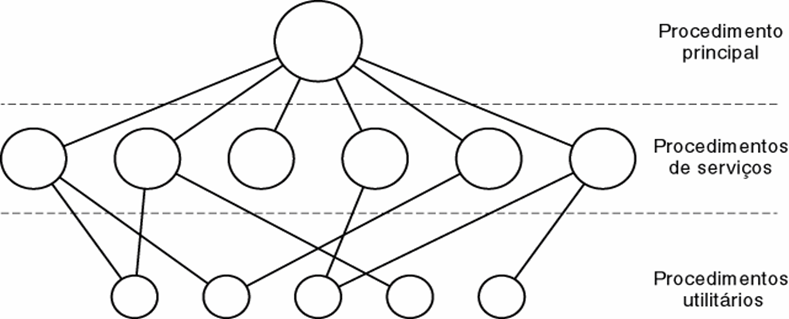
\includegraphics[width=0.9\linewidth]{assets/aula-tads-sope/SO-monolitico-1.png} % Substitua 'nome_da_imagem.jpg' pelo nome real da sua imagem
    \end{center}
\end{frame}
\begin{frame}{Sistemas Monolíticos}
    %   Neste tipo de estrutura, o SO é escrito como uma coleção de rotinas, onde cada rotina pode chamar qualquer outra rotina, sempre que for necessário.
    %   Portanto, o sistema é estruturado de forma que as rotinas podem interagir livremente umas com as outras. Quando esta técnica é usada, cada rotina no sistema possui uma interface bem definida em termos de parâmetros e resultados.

    \vspace{1cm}
    \begin{center}
        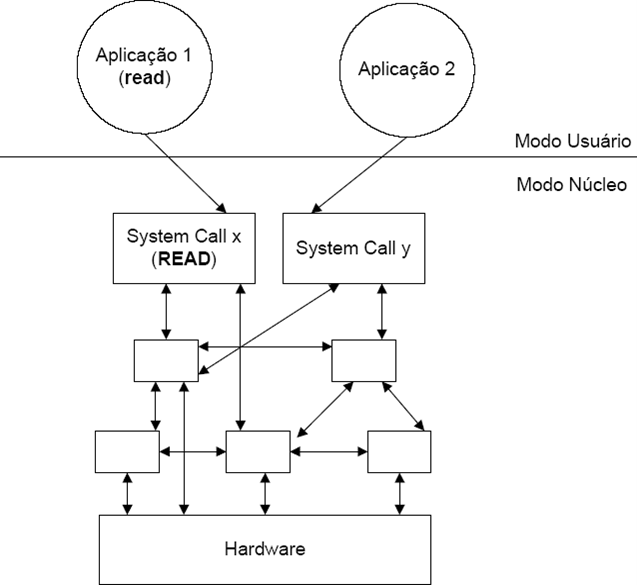
\includegraphics[width=0.45\linewidth]{assets/aula-tads-sope/SO-monolitico-2.png} % Substitua 'nome_da_imagem.jpg' pelo nome real da sua imagem
    \end{center}
\end{frame}

\begin{frame}{Sistemas Monolíticos}
    %   Neste tipo de estrutura, o SO é escrito como uma coleção de rotinas, onde cada rotina pode chamar qualquer outra rotina, sempre que for necessário.
    %   Portanto, o sistema é estruturado de forma que as rotinas podem interagir livremente umas com as outras. Quando esta técnica é usada, cada rotina no sistema possui uma interface bem definida em termos de parâmetros e resultados.

    \vspace{1cm}
    \begin{center}
        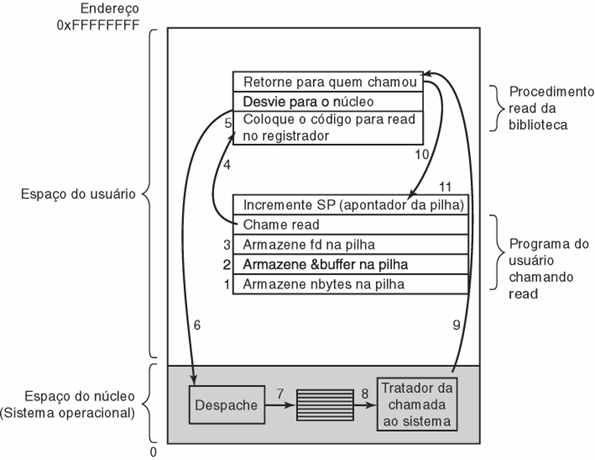
\includegraphics[width=0.5\linewidth]{assets/aula-tads-sope/SO-monolitico-3.png} % Substitua 'nome_da_imagem.jpg' pelo nome real da sua imagem
    \end{center}
\end{frame}

\section{Sistemas em Camadas}
\begin{frame}{Sistema em Camadas}
    \begin{itemize}
        \item O primeiro SO a implementar: THE
        \item THE (Technische Hogeschool Eindhoven)
        \item Holanda, 1968
        \item Construído por E. W. Dijistra e seus alunos
        \item Sistema em Lotes para o computador holandês Electrologica X8
        \item 32K de palavras de 27 bits
    \end{itemize}
\end{frame}


\begin{frame}{Sistema em camadas}
    A idéia por trás deste tipo de SO é fazer a organização por meio de hierarquia de camadas.

    \vspace{1cm}

    \begin{table}
        \centering
        \begin{tabular}{|c|l|}
            \hline
            \textbf{Camada} & \textbf{Função}                               \\
            \hline
            5               & Operador                                      \\
            \hline
            4               & Programas do usuário                          \\
            \hline
            3               & Gerenciamento de entrada e saída              \\
            \hline
            2               & Comunicação Operador-Processo                 \\
            \hline
            1               & Gerenciamentode memória e do tambor magnético \\
            \hline
            0               & Alocação de processadore multiprogramação     \\
            \hline
        \end{tabular}
    \end{table}

\end{frame}


\begin{frame}{Sistema em Camadas}
    \begin{itemize}
        \item Camada 0: Alocação do processador, alternando entre processos quando ocorriam interrupção ou temporizadores expiravam.
        \item Camada 1: Gerenciamento de memória, alocando espaços para processos na memória principal e em um tambor (antigo meio magnético de armazenamento) com 512K.
        \item Camada 2: Manipulava a Comunicação entre Processos (IPC) e o console do operador.
        \item Camada 3: Gerenciava dispositivos de E/S e armazenava em buffer os fluxos de informações.
        \item Camada 4: Os programas de usuário, não se preocupavam com gerenciamento algum (processos, memória, console ou E/S).
        \item Camada 5: Processo de operador do sistema.
    \end{itemize}
\end{frame}
\begin{frame}{Sistema THE -  Camada 0}
    O modelo de sistema em camadas propõe uma decomposição hierárquica do sistema operacional, onde cada camada fornece um conjunto de serviços para a camada imediatamente superior.

    \vspace{0.5cm}

    \textbf{Camada 0:}
    \begin{itemize}
        \item Responsável pela alocação do processador entre os processos.
        \item Chaveamento entre processos quando ocorrem interrupções ou quando os temporizadores expiram.
        \item Fornecia a multiprogramação básica da CPU.
    \end{itemize}

    \vspace{0.5cm}

    Acima da camada 0, o sistema é composto de processos sequenciais que podem ser programados sem se preocupar com a existência de múltiplos processos executando na CPU.
\end{frame}
\begin{frame}{Sistema THE -  Camada 1}
    A camada 1 é responsável pelo gerenciamento de memória no modelo de sistema em camadas.

    \vspace{0.5cm}

    \textbf{Funcionalidades da Camada 1:}
    \begin{itemize}
        \item Realiza o gerenciamento da Memória Principal.
        \item Aloca espaço para processos na Memória Principal e também em um Tambor de 512K palavras.
        \item O Tambor era utilizado para armazenar partes de processos (páginas) para as quais não havia espaço na Memória Principal.
    \end{itemize}

    \vspace{0.5cm}

    Com a camada 1 em operação, os processos acima dela não precisam se preocupar com sua localização (se estão na Memória Principal ou no Tambor). Quando necessário, a camada 1 é responsável por transferir as partes do software para a Memória Principal.
\end{frame}

\begin{frame}{Sistema THE -  Camada 2}
    A camada 2 é focada na comunicação entre o processo e o operador por meio do console.

    \vspace{0.5cm}

    \textbf{Funcionalidades da Camada 2:}
    \begin{itemize}
        \item Estabelece a interface de comunicação entre cada processo e o operador.
        \item Manipula a interação com o console que inclui:
              \begin{itemize}
                  \item Dispositivo de entrada: teclado.
                  \item Dispositivo de saída: monitor ou impressora.
              \end{itemize}
    \end{itemize}

    \vspace{0.5cm}

    Dessa forma, a camada 2 atua como uma ponte entre os processos em execução e o usuário interagindo através do console, garantindo uma comunicação eficiente e sem interrupções.
\end{frame}

\begin{frame}{Sistema THE -  Camada 3}
    A camada 3 é focada no gerenciamento dos dispositivos de Entrada e Saída (E/S).

    \vspace{0.5cm}

    \textbf{Funcionalidades da Camada 3:}
    \begin{itemize}
        \item Administra os dispositivos de E/S do sistema.
        \item Proveem uma abstração dos dispositivos de E/S para os processos.
        \item Isola os detalhes intrincados dos dispositivos reais, permitindo que os processos trabalhem com dispositivos abstratos simplificados.
    \end{itemize}

    \vspace{0.5cm}

    Com a camada 3, os processos são aliviados da complexidade de interagir diretamente com os dispositivos de hardware, possibilitando uma interação mais simplificada e eficiente.
\end{frame}

\begin{frame}{Sistema THE - Camada 4}
    A camada 4 é destinada aos programas do usuário.

    \vspace{0.5cm}

    \textbf{Características da Camada 4:}
    \begin{itemize}
        \item Oferece um ambiente para a execução dos programas de usuário.
        \item Interações diretas com o sistema operacional são mediadas pelas camadas inferiores.
        \item Garante que os programas de usuário não interfiram uns com os outros ou com o sistema operacional.
    \end{itemize}
\end{frame}
\begin{frame}{Sistema THE - Camada 5}
    A camada 5 é dedicada ao processo do operador do sistema.

    \vspace{0.5cm}

    \textbf{Funcionalidades da Camada 5:}
    \begin{itemize}
        \item Serve como interface entre o sistema e o operador.
        \item Permite que o operador inicie ou termine processos, monitore o desempenho do sistema, entre outras tarefas administrativas.
        \item Fornece ferramentas e utilitários para a manutenção e monitoramento do sistema.
    \end{itemize}

    \vspace{0.5cm}

    Esta camada é crucial para a gestão eficaz do sistema e para a manutenção da estabilidade operacional.
\end{frame}


\begin{frame}{Resumo sistema THE}
    O esquema de camadas do THE era, de fato, apenas um auxílio de desenho (design), pois todas as partes do sistema eram intimamente unidas em um único código executável.
\end{frame}


\begin{frame}{Máquinas Virtuais}
    \begin{itemize}
        \item OS/360 = sistemas em lote.
        \item Muitos usuários do sistema queriam ter tempo compartilhado.
        \item Grupos dentro e fora da IBM decidiram escrever um sistema de tempo compartilhado para o OS/360.
        \item TSS/360 = tempo compartilhado oficial da IBM.
        \item Era grande e lento e foi abandonado, custando U\$50 milhões.
    \end{itemize}
\end{frame}
\begin{frame}{Máquinas Virtuais - VM/370}
    \begin{itemize}
        \item Um grupo científico da IBM em Cambridge desenvolveu outro sistema.
        \item Esse SO foi adotado pela IBM para computadores de grande porte.
        \item Originalmente chamava-se CP/M, mas depois foi renomeado para VM/370.
        \item Projetado com dois módulos principais:
              \begin{itemize}
                  \item Multiprogramação
                  \item Máquina Estendida
              \end{itemize}
    \end{itemize}
\end{frame}
\begin{frame}{Máquina Virtual - Monitor da VM}
    \begin{itemize}
        \item O centro do SO era conhecido como Monitor de Máquina Virtual.
        \item Executava-se no hardware básico e implementava a multiprogramação.
        \item Oferecia várias máquinas virtuais, que eram cópias exatas do hardware básico.
        \item Incluía os modos kernel e usuário, proporcionando isolamento e proteção entre as VMs.
        \item Preservava todos os detalhes originais da máquina real em cada VM.
    \end{itemize}
\end{frame}
\begin{frame}{Máquina Virtual}
    \begin{itemize}
        \item As máquinas virtuais podem executar sistemas operacionais distintos.
        \item Exemplo:
              \begin{itemize}
                  \item Algumas VMs rodavam descendentes do OS/360 para processamento em lote.
                  \item Outras executavam o CMS (Conversational Monitor System) para tempo compartilhado.
              \end{itemize}
        \item O conceito de máquinas virtuais também é empregado nos processadores compatíveis com x86, como o \textbf{Modo Virtual 8086}.
    \end{itemize}
\end{frame}


\section{Modelo Cliente - Servidor}
\begin{frame}{Modelo Cliente-Servidor}
    \begin{itemize}
        \item Mover recursos do SO para fora do kernel.
        \item Deixando um núcleo mínimo: \textbf{Microkernel}.
        \item Implementar funções do SO como processos em modo usuário.
        \item Existe uma abordagem de processo cliente e processo servidor.
        \item O núcleo gerencia a comunicação entre clientes e servidores.
    \end{itemize}
\end{frame}
\begin{frame}{Modelo Cliente-Servidor}
    \begin{itemize}
        \item Os processos executando em modo usuário não têm acesso direto ao hardware.
        \item A consequência disso é que se ocorrer um erro no servidor de arquivos (por exemplo), não derrubará a máquina inteira.
        \item Capacidade de adaptação para uso em Sistemas Distribuídos.
    \end{itemize}
\end{frame}
\begin{frame}{Sistemas Cliente - Servidor - Arquitetura }
    Uma tendência dos sistemas operacionais modernos é transferir códigos para as camadas mais superiores e remover o máximo possível de código em modo núcleo, deixando um micronúcleo mínimo (também chamado de microkernel).
\end{frame}

\begin{frame}{Sistemas Cliente - Servidor- Arquitetura }
    Normalmente, se implementa o máximo do sistema operacional como um processo do usuário. Para requisitar um serviço, como ler um bloco de arquivo, um processo de usuário (agora conhecido como processo cliente), envia uma requisição para um processo servidor, que então executa o trabalho e envia a resposta.
\end{frame}
\begin{frame}{Sistemas Cliente - Servidor- Arquitetura}
    %   Neste tipo de estrutura, o SO é escrito como uma coleção de rotinas, onde cada rotina pode chamar qualquer outra rotina, sempre que for necessário.
    %   Portanto, o sistema é estruturado de forma que as rotinas podem interagir livremente umas com as outras. Quando esta técnica é usada, cada rotina no sistema possui uma interface bem definida em termos de parâmetros e resultados.

    \vspace{1cm}
    \begin{center}
        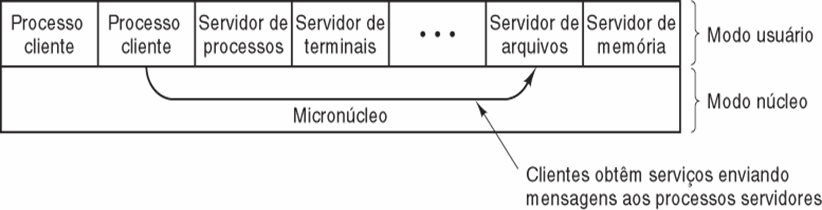
\includegraphics[width=0.8\linewidth]{assets/aula-tads-sope/SO-cli-ser-1.png} % Substitua 'nome_da_imagem.jpg' pelo nome real da sua imagem
    \end{center}
\end{frame}
\begin{frame}{Sistemas Cliente - Servidor}
    Como mostra a figura anterior, tudo o que o núcleo faz é tratar da comunicação entre clientes e servidores, dividindo o sistema operacional em várias partes:

    \begin{itemize}
        \item servidor de arquivos;
        \item servidor de processos;
        \item servidor de terminais;
        \item servidor de memória;
    \end{itemize}

    Todos esses processos executam em modo usuário. Assim, se algum problema ocorrer, o sistema não será danificado.
\end{frame}

\begin{frame}{Sistemas Cliente - Servidor e Adaptabilidade}
    O sistema cliente-servidor possui uma adaptabilidade ao uso em sistemas distribuídos. Ao comunicar-se com um processo servidor enviando-lhe uma mensagem, o cliente não precisa saber:

    \begin{itemize}
        \item Se esta mensagem será tratada localmente;
        \item Se será tratada remotamente.
    \end{itemize}

    Essa abstração proporciona flexibilidade na distribuição de serviços no sistema.
\end{frame}

\begin{frame}{Sistemas Cliente - Servidor- Arquitetura}
    %   Neste tipo de estrutura, o SO é escrito como uma coleção de rotinas, onde cada rotina pode chamar qualquer outra rotina, sempre que for necessário.
    %   Portanto, o sistema é estruturado de forma que as rotinas podem interagir livremente umas com as outras. Quando esta técnica é usada, cada rotina no sistema possui uma interface bem definida em termos de parâmetros e resultados.

    \vspace{1cm}
    \begin{center}
        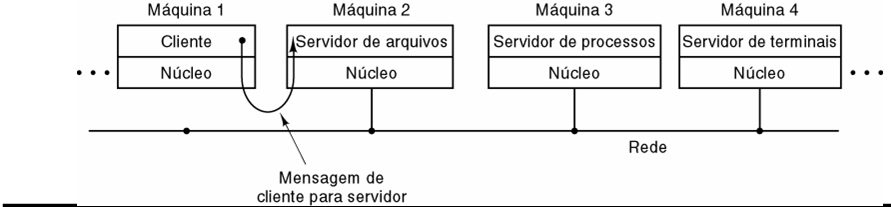
\includegraphics[width=0.9\linewidth]{assets/aula-tads-sope/SO-cli-ser-2.png} % Substitua 'nome_da_imagem.jpg' pelo nome real da sua imagem
    \end{center}
\end{frame}
\begin{frame}{Sistemas Cliente – Servidor X Sistemas monolíticos: Visão Geral}
    Em uma primeira análise, uma estrutura de SO Cliente-Servidor parece ser bem melhor do que um SO Monolítico.
    \begin{itemize}
        \item SO Cliente-Servidor: Mais modular e abstrato.
        \item SO Monolítico: Todo o controle reside no Modo Núcleo.
    \end{itemize}
\end{frame}

\begin{frame}{Desafios da Estrutura Cliente-Servidor}
    Implementar uma estrutura Cliente-Servidor é complicado:
    \begin{itemize}
        \item Algumas funções do SO exigem acesso direto ao hardware, como operações de E/S.
        \item Complexidade maior em gerenciar comunicações e solicitações.
    \end{itemize}
\end{frame}

\begin{frame}{Vantagens do Núcleo Monolítico}
    Um núcleo Monolítico possui:
    \begin{itemize}
        \item Complexidade menor.
        \item Todo o código de controle reside em um único espaço de endereçamento.
        \item Performance otimizada.
    \end{itemize}
\end{frame}

\begin{frame}{Debate Histórico: Torvalds vs Tanenbaum}
    Um aspecto interessante foi a discussão entre:
    \begin{itemize}
        \item Linus Torvalds: Criador do Linux.
        \item Andrew Tanenbaum: Pesquisador em SOs, criador do Minix.
    \end{itemize}
    Em 1992, Tanenbaum criticou o Linux por ser Monolítico, considerando-o obsoleto.
\end{frame}







\section{Estudo de caso - Windows 2000/NT}
\begin{frame}{O Windows 2000: Contexto Histórico}
    A história do Windows NT teve início com o desejo da Microsoft de inovar:
    \begin{itemize}
        \item Explorar inovações tecnológicas dos processadores no final da década de 80 e início de 90.
        \item Criar um sistema operacional multitarefa para ambientes monousuário e multiusuário.
    \end{itemize}
\end{frame}

\begin{frame}{Origens do Nome e Design}
    \begin{itemize}
        \item O nome "Windows" provém do sistema de janelas (Windows 3.x for Workgroup) para competir com a interface dos Macintosh (Apple).
        \item Esse ambiente emprestou sua "aparência" para o Windows NT.
        \item "NT" significa "New Technology", indicando a nova filosofia que guiou sua concepção.
    \end{itemize}
\end{frame}

\begin{frame}{Lançamento e Características do Windows NT}
    \begin{itemize}
        \item Primeira versão do Windows NT (3.1) lançada em 1993.
        \item Primeiro sistema operacional de 32 bits da Microsoft.
        \item Oferecia compatibilidade com o MS-DOS e aplicações para o Windows 3.x for Workgroup.
    \end{itemize}
\end{frame}
\begin{frame}{Evolução do Windows NT}
    \begin{itemize}
        \item Após o Windows NT 3.x, surge o Windows NT 4.0.
        \item Arquitetura do NT 4.0 semelhante à do NT 3.x.
        \item Mudanças notáveis na interface gráfica e migração de serviços do subsistema Win32 para o núcleo.
    \end{itemize}
\end{frame}

\begin{frame}{O Nascimento do Windows 2000}
    \begin{itemize}
        \item Lançado em 1999, também conhecido como Windows NT 5.0.
        \item Estrutura similar ao NT 4.0.
        \item Foco em serviços para ambientes distribuídos e de rede.
    \end{itemize}
\end{frame}

\begin{frame}{Versões do Windows 2000}
    \begin{itemize}
        \item Windows 2000 Professional: substitui o NT workstation.
        \item Windows 2000 Server: para compartilhamento de recursos em redes.
        \item Windows 2000 Advanced Server: foco em redes e ambientes distribuídos.
        \item Windows 2000 Datacenter Server: suporta até 64 GB e tem todas as funcionalidades do Win 2000.
    \end{itemize}
\end{frame}

\begin{frame}{Objetivos do Desenvolvimento do Windows 2000}
    Cinco principais objetivos:
    \begin{enumerate}
        \item Confiabilidade e robustez.
        \item Extensibilidade e facilidade de manutenção.
        \item Portabilidade.
        \item Desempenho.
        \item Conformidade com o padrão POSIX.
    \end{enumerate}
\end{frame}

\begin{frame}{Detalhes dos Objetivos}
    \begin{itemize}
        \item Confiabilidade e robustez: proteção contra mal funcionamento e ataques.
        \item Extensibilidade e manutenção: adaptabilidade às novas necessidades de hardware e software.
    \end{itemize}
\end{frame}
\begin{frame}{Arquitetura do Windows 2000: Introdução}
    \begin{itemize}
        \item Um SO é um software complexo, com modelos que variam de kernel monolítico a micronúcleo.
        \item Windows 2000 inspirado no princípio de micronúcleo.
        \item Cada funcionalidade gerenciada por um componente único.
        \item Componentes interagem através de interfaces bem definidas.
    \end{itemize}
\end{frame}

\begin{frame}{Windows 2000: Micronúcleo e Modo Protegido}
    \begin{itemize}
        \item Não é puramente orientado à filosofia micronúcleo.
        \item Módulos fora do micronúcleo executam operações em modo protegido.
        \item Decisão baseada em desempenho para evitar trocas frequentes de contexto.
    \end{itemize}
\end{frame}

\begin{frame}{Organização em Camadas e Modelo Orientado a Objetos}
    \begin{itemize}
        \item SO dividido em módulos dispostos em camadas.
        \item Cada camada oferece serviços à superior e utiliza serviços da inferior.
        \item Recursos do sistema são objetos manipulados por métodos associados.
    \end{itemize}
\end{frame}

\begin{frame}{Estrutura do Windows 2000}
    \begin{itemize}
        \item Dividido em modo usuário (subsistemas protegidos) e modo kernel (o executivo).
        \item Subsistemas interagem através de LPC (Local Procedure Call).
        \item No modo kernel, componentes interagem com hardware diretamente.
        \item Orientação a objetos protege componentes uns dos outros.
    \end{itemize}
\end{frame}

\begin{frame}{Modo Kernel e Componentes Principais}
    \begin{itemize}
        \item Estruturado em: hardware abstraction layer(HAL), drivers de dispositivos e o executivo.
        \item HAL é um módulo carregável do núcleo.
        \item A figura (não fornecida) mostra a arquitetura completa.
    \end{itemize}
\end{frame}


\begin{frame}{Estrutura do Windows NT}
    \begin{center}
        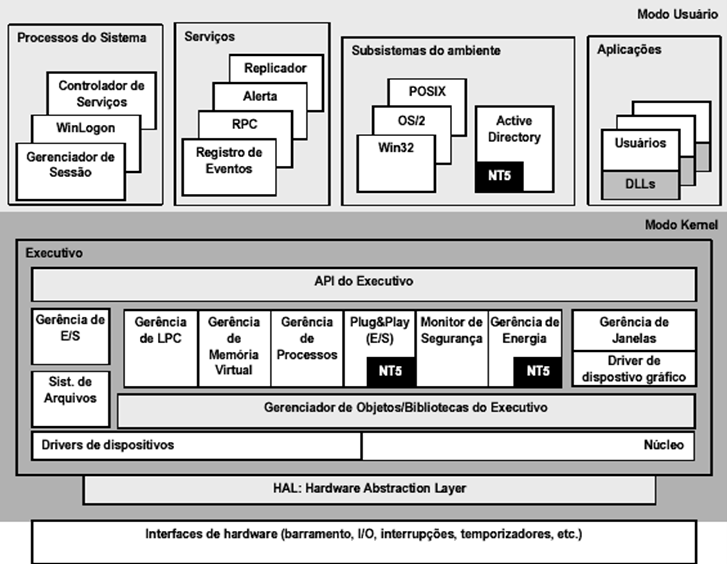
\includegraphics[width=0.6\linewidth]{assets/aula-tads-sope/SO-win-nt.png} % Substitua 'nome_da_imagem.jpg' pelo nome real da sua imagem
    \end{center}
\end{frame}


\section{Estudo de caso - UNIX/LINUX}
\begin{frame}{Origens do Unix}
    \begin{itemize}
        \item Relação direta com o sistema operacional Multics da década de 1960.
        \item Projeto conjunto: MIT, GE, Bell Labs e AT\&T.
        \item Multics possuía características de tempo compartilhado, sendo avançado para sua época.
    \end{itemize}
\end{frame}

\begin{frame}{Nascimento do Unix}
    \begin{itemize}
        \item Ken Thompson, pesquisador da Bell Labs, estava envolvido no projeto Multics.
        \item Após Bell Labs se retirar do projeto, Thompson continuou trabalhando em suas ideias.
        \item Intenção: Criar algo menor que o Multics, mas mantendo suas ideias principais.
    \end{itemize}
\end{frame}

\begin{frame}{Nomeação e Desenvolvimento}
    \begin{itemize}
        \item Brian Kernighan, pesquisador da Bell Labs, nomeou o novo sistema como "Unix".
        \item O Unix influenciou o desenvolvimento de muitos sistemas operacionais subsequentes, incluindo o Linux.
    \end{itemize}
\end{frame}
\begin{frame}{Primeira Versão do Unix}
    \begin{itemize}
        \item Originalmente escrito em linguagem assembler.
        \item Em 1973, Dennis Ritchie reescreveu o Unix em C, uma linguagem de alto nível por ele desenvolvida.
        \item Esta mudança aumentou significativamente a aceitação do Unix por usuários externos à Bell Labs.
    \end{itemize}
\end{frame}

\begin{frame}{Desenvolvimentos no Unix: Década de 1980}
    \begin{itemize}
        \item 1980: Universidade da Califórnia em Berkeley recebeu financiamento para desenvolver um Unix para computação distribuída, resultando no 4.1 BSD.
        \item Início dos anos 80: Microsoft lançou XENIX, uma versão comercial do Unix, que mais tarde evoluiu para SCO-Unix.
    \end{itemize}
\end{frame}

\begin{frame}{Lançamentos e Licenças da AT\&T}
    \begin{itemize}
        \item 1982: AT\&T introduziu o UNIX System III.
        \item Evoluiu para o System V.
        \item Devido a restrições legais, AT\&T licenciou o System V para outras empresas e institutos de pesquisa.
    \end{itemize}
\end{frame}
\begin{frame}{Desenvolvimento pela Sun Microsystems}
    \begin{itemize}
        \item Sun Microsystems lança sua versão do UNIX chamada SunOS, baseada no 4.2 BSD de Berkeley.
        \item Introdução do Network File System (NFS) permitindo compartilhamento de arquivos em redes locais.
    \end{itemize}
\end{frame}

\begin{frame}{Diversidade do UNIX no final dos anos 80}
    \begin{itemize}
        \item Duas grandes "famílias" de UNIX: 4.3 BSD e System V Release 3.
        \item Fabricantes incorporavam suas próprias melhorias.
        \item Incompatibilidades surgem entre as diferentes versões.
    \end{itemize}
\end{frame}



\begin{frame}{Busca pela Padronização}
    \begin{itemize}
        \item Tentativas feitas para padronizar as interfaces do UNIX.
        \item Objetivo: Facilitar o porte de aplicações entre as diversas versões.
        \item Sucesso na padronização alcançado pelo IEEE Standards Board com o padrão POSIX.
        \item POSIX define funções de biblioteca essenciais para todos os sistemas que o adotam.
    \end{itemize}
\end{frame}
\begin{frame}{Origens do Linux nos Anos 90}
    \begin{itemize}
        \item Linus Torvalds busca desenvolver núcleo de SO para o Intel 386.
        \item Baseado no Minix, um SO didático.
    \end{itemize}
\end{frame}

\begin{frame}{Evolução para o UNIX Open Source}
    \begin{itemize}
        \item Sistema evolui e se torna versão de UNIX.
        \item Distribuído em modalidade open source.
        \item Código-fonte disponível gratuitamente para download e distribuição.
    \end{itemize}
\end{frame}

\begin{frame}{Breve genealogia dos Sistemas apresentados}
    \begin{center}
        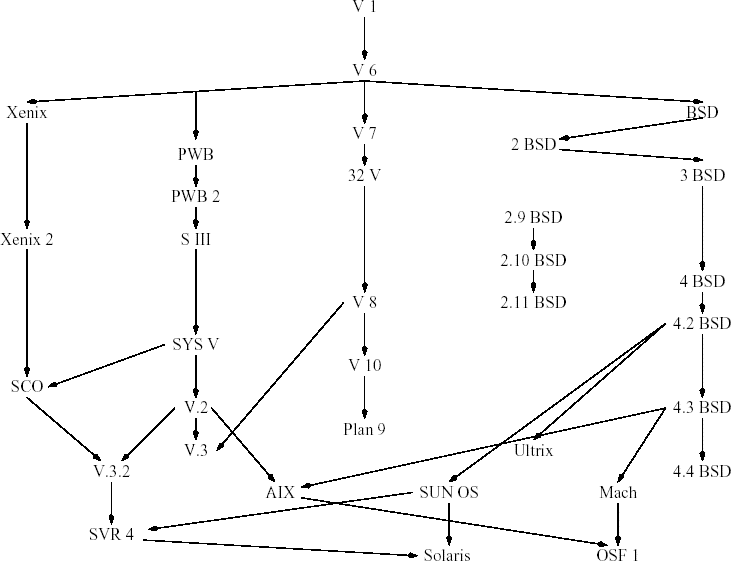
\includegraphics[width=0.55\linewidth]{assets/aula-tads-sope/SO-unix-linux-1.png}
    \end{center}
\end{frame}



\begin{frame}{Disseminação do Linux}
    \begin{itemize}
        \item Rápida disseminação global do Linux.
        \item Ganhando popularidade em instalações domésticas e institucionais.
    \end{itemize}
\end{frame}
\begin{frame}{Estrutura do UNIX/LINUX}
    \begin{itemize}
        \item Kernel Monolítico: Todas funcionalidades em modo núcleo.
        \item Acesso completo a rotinas e estruturas de dados internas.
    \end{itemize}
\end{frame}

\begin{frame}{Desafios do Kernel Monolítico}
    \begin{itemize}
        \item Qualquer mudança exige reconstrução completa do kernel.
        \item Adição de drivers ou funcionalidades implica em recompilação.
        \item Processo trabalhoso e demorado.
    \end{itemize}
\end{frame}
\begin{frame}{Base monolítica do UNIX/Linux}
    O Unix como o Linux é baseado em estrutura monolítica.
    
    \begin{center}
        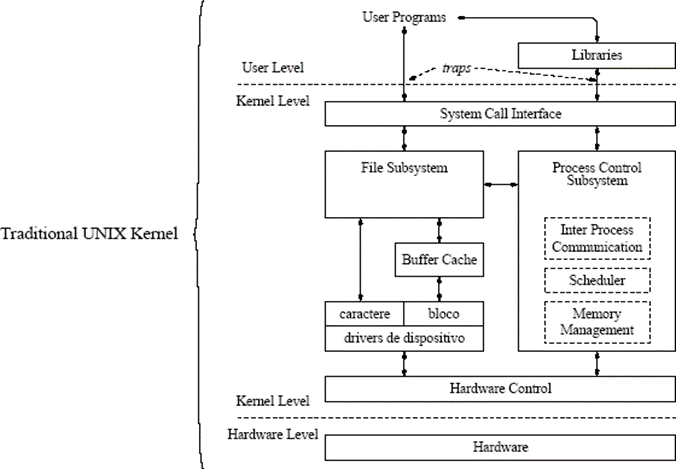
\includegraphics[width=0.6\linewidth]{assets/aula-tads-sope/SO-unix-linux-2.png}
    \end{center}
\end{frame}
\begin{frame}{Visão da arquitetura do UNIX}
    
    \begin{center}
        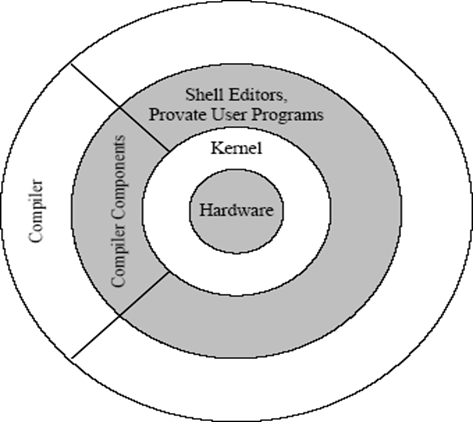
\includegraphics[width=0.45\linewidth]{assets/aula-tads-sope/SO-unix-linux-3.png}
    \end{center}
\end{frame}
\begin{frame}{Solução: Loadable Modules}
    \begin{itemize}
        \item Blocos independentes de código.
        \item Solução para problemas de reconstrução do kernel.
        \item Características principais:
            \begin{itemize}
                \item Dynamic linking.
                \item Stackable linking.
            \end{itemize}
    \end{itemize}
\end{frame}

\begin{frame}{Características dos Loadable Modules}
    \begin{itemize}
        \item Módulos carregados e linkados enquanto kernel está em execução.
        \item Hierarquia de módulos permite modularidade e flexibilidade.
        \item Módulos funcionam como bibliotecas para módulos clientes.
    \end{itemize}
\end{frame}

\begin{frame}{Manipulando Módulos no Linux}
    \begin{itemize}
        \item Dynamic linking facilita configuração.
        \item Comandos para gerenciar módulos:
            \begin{itemize}
                \item insmod: carregar módulo.
                \item modprobe: carregar módulo com dependências.
                \item rmmod: remover módulo.
            \end{itemize}
    \end{itemize}
\end{frame}
\begin{frame}{Visão da arquitetura em módulos}
    
    \begin{center}
        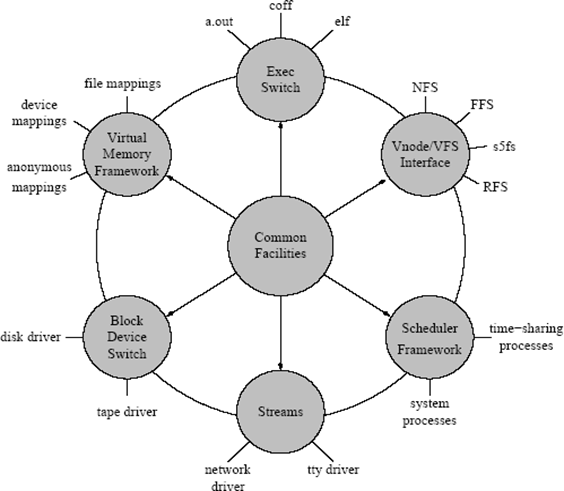
\includegraphics[width=0.5\linewidth]{assets/aula-tads-sope/SO-unix-linux-4.png}
    \end{center}
\end{frame}




\begin{frame}{Referências }\justifying
    \begin{itemize}
        \item \textbf{Slides SOPA2 - Prof. Alexandre Beletti Ferreira}
        \item \textbf{TANENBAUM, Andrew S.; WOODHULL, Albert S.} Sistemas operacionais: projeto e implementação. 3. ed. Porto Alegre: Bookman, 2008. ISBN 9788577800571.
    \end{itemize}
\end{frame}

\begin{frame}[fragile]{Imagem do dia}

    \begin{figure}[H]
        \centerline{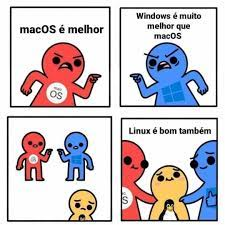
\includegraphics[width=0.4\textwidth]{assets/imagem-do-dia/sope-02.jpeg}}

    \end{figure}
\end{frame}

\backmatter
\end{document}
